\documentclass{article}
\renewcommand{\thesection}{}
\usepackage[polish]{babel}
\usepackage[T1]{fontenc}
\usepackage{geometry}
\usepackage{chngpage}
\usepackage{graphicx}
\usepackage{subcaption}
\usepackage{float}
\usepackage{amsfonts}
\usepackage{amsmath}
\geometry{margin=2cm}
\usepackage[utf8]{inputenc}
\usepackage{indentfirst}
\usepackage{longtable}
\usepackage{gensymb}
\frenchspacing
\setlength{\parindent}{3em}
\begin{document}
\section{\centering Zadanie 3}
Pokaż, że w każdym grafie prostym o co najmniej dwóch wierzchołkach są dwa wierzchołki o takim samym rzędzie. \\\\
ODP:\\
Niech $G = (V,E)$ i $n = |V|$. Musimy rozważyć dwa przypadki:\\
\begin{itemize}
	\item Istnieje izolowany wierzchołek: \\\\ Niech a będzie wierzchołkiem izolowanym. Wtedy dla dowolnego $x \in V \textbackslash \{a\}$ mamy $\mathcal{N}(x)  \subseteq V \textbackslash \{a,x\}$, więc $deg(x) \leq n-2$. Zatem deg : $V \rightarrow \{0,...n-2\}$. Ale $|V| =n$ i $|\{0,...,n-2\}| = n-1$, więc deg nie jest injekcją
	\item Nie istnieje wierzchołek izolowany: \\\\ Wtedy deg : $V \rightarrow \{1,...,n-1\}$, zatem deg nie jest injekcją\\\\
\end{itemize}
\noindent \textbf{DEF}:\\
\textbf{$\mathcal{N}$} - Sąsiedzi wierzchołka - dla $G = G(D,C)$ i $X \subseteq D$ mamy $\mathcal{N}(X) = \{y \in C : (\exists x \in X)(\{x,y\} \in E(G))\}$\\
\section{\centering Zadanie 4}
Pokaż, że graf cykliczny $C_{n}$ jest grafem dwudzielnym wtedy i tylko wtedy, gdy $n$ jest liczbą parzystą \\\\
ODP:\\
Jeżeli $n = 2k$ to $C_{n}$ rozkłada się na dwa zbiory: $X = \{1,3,...,2k-1\}$ i $Y = \{2,4,...,2k\}$ - za darmo.\\\\
Jeżeli n nie jest parzyste to wystarczy skorzystać z charakteryzacji grafów dwudzielnych - są to grafy których wszystkie cykle są długości parzystej - nie da się takich stworzyć dla n nieparzystego więc sprzeczność.

\section{\centering Zadanie 5}
Wyznacz średnicę i rzędy elementów w hiperkostce $Q_{n}$.\\\\
ODP:\\
Hiperkostka powstaje poprzez podwajanie ilości elementów hiperkostrki o stopniu o 1 mniejszym.\\\\
Tj:\\
$deg(Q) = n$\\
$d(Q) = n$ (najdłuższa najkrótsza ścieżka)\\\\
d-d:\\
$deg(Q_1) = 1$\\
$d(Q_1) = 1$\\
$Q_n \cong G \cong G'$, gdzie $G = (V, E)$, $G' = (V', E')$\\
wtedy $Q_{n+1} = (V \cup V', E \cup E' \cup {(v_k, v'_k): v_k \in V \wedge v'_k \in V' \wedge 0 \leq k < 2^n})$\\
$d(Q_{n+1}) = max(dist(v_1, v_2): v_1,v_2 \in V \cup V')$\\
dla $v_k \in V, v'_l \in V'$, $dist(v_k, v'_l) = dist(v_k, v_l) + dist(v_l, v'_l) = dist(v_k, v_l) + 1$\\
więc $d(Q_{n+1}) = max(dist(v_k, v_l) + 1) = max(dist(v_k, v_l)) + 1 = d(Q_n) + 1$\\\\
kiedy łączymy dwa $Q_n$ w $Q_{n+1}$, to do każdego wierzchołka dodajemy dokładnie jedną krawędź\\
więc $deg(Q_{n+1}) = deg(Q_n) + 1$\\\\
\section{\centering Zadanie 6 }
Pokaż, że dla każdego $n \geq 1$ hiper-kostka $Q_{n}$ jest grafem dwudzielnym.\\\\
ODP:\\
$Q_n = (V, E)$\\
Zdefiniujmy funkcję $f: V \rightarrow \{ 0,1\} ^n$\\
$(v_1, v_2) \in E \Leftrightarrow f(v_1) \verb| i | f(v_2) \verb| różnią się tylko 1 elementem|$\\
wtedy $(v_1, v_2) \in E \Rightarrow sum(f(v_1)) = sum(f(v_2)) \pm 1$\\
weźmy $V = V_1 \cup V_2$\\
$V_1 = \{ v \in V: \neg (2 \mid sum(f(v)))\} $\\
$V_2 = \{ v \in V: 2 \mid sum(f(v))\} $\\
widać że $V_1$ i $V_2$ są rozłączne\\
wtedy $v_1,v_2 \in V_1 \lor v_1, v_2 \in V_2 \implies sum(f(v_1)) = sum(f(v_2)) \pm 2k$\\
czyli $(v_1,v_2) \notin E$\\
więc graf jest dwudzielny\\\\
\section{\centering Zadanie 13}
Rozstrzygnij czy następujące ciągi są graficzne i jeśli ciąg jest graficzny, to znajdź graf prosty o tym ciągu stopni: \\\\
1. (4,3,2,1,0) \hspace{1cm} 2 .(4,3,3,2,2,1,1) \hspace{1cm} 3. (6,4,4,4,3,1,1,1) \\\\
Punkt (1): nie ma takiego grafu; oto uzasadnienie: graf taki musiałby mieć 5 wierzchołków i jeden z nich miałby rząd 4; miałby więc on krawędź ze wszystkimi innymi; więc żaden wierzchołek nie może mieć rzędu 0.\\\\
Przykłady z punktów (2) i (3) zbudować można tak: bierzemy rozważany ciąg; stosujemy twierdzenie Havela-Hakimi tak długo aż otrzymamy ciąg rzędów dla którego potrafimy znaleźć odpowiadający im graf a potem odwracamy proces.\\\\
\textbf{TW. HAVELA-HAKIMI} - Ciąg ($d_{1},...,d_{n}$) jest graficzny tylko wtedy gdy ciąg ($d'_{1},...,d'_{n}$) jest graficzny, gdzie:
\begin{equation}
d'_{i}=\begin{cases}
d_{i} - 1  & \text{: i=2, ..., $d_{1}$ + 1}\\
d_{i}   & \text{: i = $d_{1}$ + 2, ..., n}
\end{cases}
\end{equation}
\begin{figure}[ht]
	\begin{subfigure}{.5\textwidth}
		\centering
		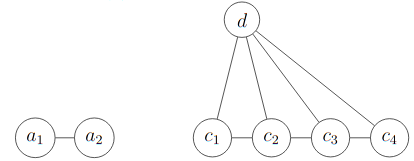
\includegraphics[width=.6\linewidth]{z13_p2.png}  
		\caption*{ppunkt 2}
		
	\end{subfigure}
	\begin{subfigure}{.5\textwidth}
		\centering
		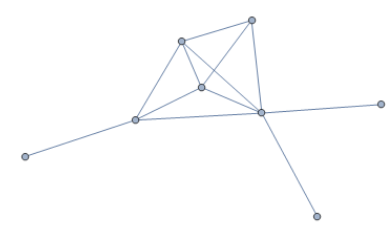
\includegraphics[width=.6\linewidth]{z13_p3.png}  
		\caption*{ppunkt 3}
		
	\end{subfigure}
\end{figure}
\section{\centering Zadanie 14}
Pokaż, że grafy proste $G_{1}$ i $G_{2}$ są izomorficzne wtedy i tylko wtedy, gdy ich dopełnienia $\overline{G_{1}}$ i $\overline{G_{2}}$ są izomorficzne. \\\\
ODP:\\
Niech $G_{1} = (V_{1}, E_{1})$ i $G_{2} = (V_{2}, E_{2})$ oraz niech $f:V_{1} \rightarrow V_{2}$ będzie izomorfizmem grafów. Wtedy dla dowolnych $x,y \in V_{1}$ mamy:\\\\
${x,y} \in E(G_{1}) \iff {f(x),f(y)} \in E(G_{2})$, więc\\
${x,y} \notin E(G_{1}) \iff {f(x),f(y)} \notin E(G_{2})$, czyli\\
${x,y} \in E(\overline{G_{1}}) \iff {f(x),f(y)} \in E(\overline{G_{2}})$
\section{\centering Zadanie 25}
Załóżmy że $G = (V,E)$ jest takim grafem prostym że $|E| \geq |V|$. Pokaż że graf G zawiera cykl.\\\\
Drzewo - $G = (V,E), |V| = n, |E| = n-1$ \\
ODP: \\ Weźmy przypadek graniczny - drzewo z jedną dodaną krawędzią. Nie można dodać krawędzi do drzewa w taki sposób aby nie stworzyć cyklu.
\section{\centering Zadanie 26}
Niech $G = (V,E)$ będzie grafem prostym. Załóżmy że  $v \in V$ jest wierzchołkiem o stopniu nieparzystym. Pokaż że istnieje inny wierzchołek $u \in V$ o rzędzie nieparzystym od którego jest jakaś droga do $v$. \\\\
ODP: \\
Tw Eulera: $\sum_{v \in V}deg(v) = 2 * |E|$ \\\\
Suma stopnie wierzchołków spójnych składowych jest parzysta, a więc jeżeli $v,u \in V$ w grafie spójnym to musi istnieć między nimi droga
\\\\
\section{\centering Zadanie 29}
\begin{figure}[H]
	\centering
	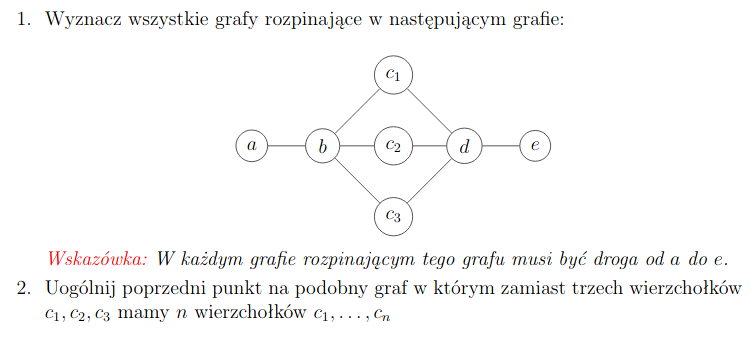
\includegraphics[width=0.9\linewidth]{z29.png}  
\end{figure}
\noindent ODP: \\
Dla $n$ wierzchołków $c_{1},....,c_{n}$ mamy $n * 2^{n-1}$\\\\
\noindent \textbf{DEF}:\\
Graf rozpinający to inaczej drzewo rozpinające. 
\section{\centering Zadanie 33}
Wyznacz liczbę grafów rozpinających w grafach $K_{2,n}$ \\\\

$K_{2,3}$: \\
\begin{figure}[H]
	\centering
	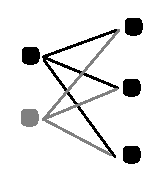
\includegraphics[width=0.1\linewidth]{z33_1.png}  
\end{figure}
to to samo co: \\
\begin{figure}[H]
	\centering
	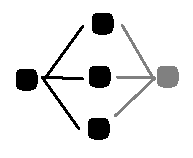
\includegraphics[width=0.1\linewidth]{z33_2.png}  
\end{figure}
%\begin{figure}[H]
%	\centering
%	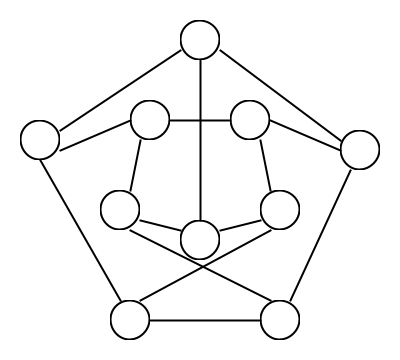
\includegraphics[width=0.3\linewidth]{z45.png}  
%\end{figure}
Wiec liczba grafów rozpinających to $n * 2^{n-1}$\\\\
\noindent \textbf{DEF:} \\
$K_{2,n}$ - pełen graf dwudzielny \\
\section{\centering Zadanie 35}
Niech $T$ będzie drzewem. Pokaż, że $\overline{d}(T) \leq 2$ ($\overline{d}(T)$ - średni stopień wierzchołka w $T$)\\\\
ODP:\\
Tw Eulera: $\sum_{v \in V}deg(v) = 2 * |E|$ \\
Z tw. Eulera wiadomo, że dla drzewa suma wszystkich stopni wierzchołków to $2n-2$ (dwukrotność liczby krawędzi)\\\\
$\frac{2*n-2}{n} = 2 - \frac{2}{n} \leq 2$\\\\
\section{\centering Zadanie 37}
Pokaż że $\delta(G) \leq \overline{d}(G) \leq \Delta(G)$ \\\\
ODP: \\
$\forall x \in G$ $deg(x) \geq \delta(G)$, więc
$$\overline{d}(G) = \frac{\sum_{x \in V(G)}deg(x)}{|V(G)|} \geq \frac{\sum_{x \in V(G)}\delta(G)}{|V(G)|}$$
$\forall x \in G$ $deg(x) \leq \Delta(G)$, więc
$$\overline{d}(G) = \frac{\sum_{x \in V(G)}deg(x)}{|V(G)|} \leq \frac{\sum_{x \in V(G)}\Delta(G)}{|V(G)|}$$
\noindent \textbf{DEF:} \\
$\Delta(G)$ - $max\{deg(x) : x \in V(G)\}$\\
$\delta(G)$ - $min\{deg(x) : x \in V(G)\}$
\section{\centering Zadanie 45}
Narysuj na płaszczyźnie graf Petersena tak aby na rysunku były tylko dwa przecięcia krawędzi. \\\\
ODP: \\
\begin{figure}[H]
	\centering
	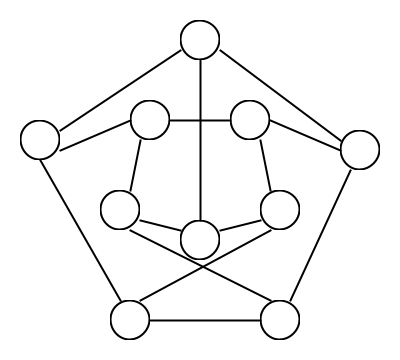
\includegraphics[width=0.3\linewidth]{z45.png}  
\end{figure}
\section{\centering Zadanie 49}
Wyznacz liczby $\kappa(G)$, $\lambda(G)$, $\delta(G)$ dla grafów $K_{n}$, $L_{n}$ oraz $W_{n}$ (dla wszystkich $n$): \\\\
ODP: \\

\begin{tabular}{p{2cm}|p{2cm}|p{2cm}|p{2cm}}
  & $\delta(G)$ & $\kappa(G)$ & $\lambda(G)$  \\
  	\hline
 	$K_{n}$ & n-1 & n-1 & n-1  \\
 	\hline
  	$L_{n}$ & 1 & 1 & 1  \\
  	\hline
  	$W_{n}$ & 3 & 3 & 3  \\
\end{tabular}\\\\
\noindent \textbf{DEF:} \\
$\lambda(G)$ - Spójność krawędziowa grafu spójnego $G=(V,E)$, \\ 
\indent $\lambda(G) = min \{|Y|: (Y \subseteq E) \land (G\textbackslash Y$ nie jest spójny$)\}$\\\\
$\delta(G)$ - Minimalny rząd wierzchołka grafu:\\
\indent $\delta(G) = min\{deg(x) : x \in V(G)\}$\\\\
$\kappa(G)$ - Spójność wierzchołkowa grafu spójnego:\\
\indent $\kappa(G)$ = 
$\begin{cases}
n - 1  & \text{: G \textasciitilde $K_{n}$}\\
min\{|X| : X \subseteq V \land G \textbackslash X$ nie jest spójny$   & \text{: nie jest pełny} 
\end{cases}$
,gdzie $K_{n}$ - graf pełny\\\\\\
\textbf{Graf pełny} $K_n$  to graf prosty, w którym dla każdej pary wierzchołków istnieje krawędź je łącząca. Jeżeli graf pełny ma |V|=n wierzchołków, to posiada $|E|=n(n-1)/2$ krawędzi. Graf pełny jest grafem regularnym stopnia n-1.\\
\textbf{Graf koło} $W_n$ to graf powstający z grafu $C_{n-1}$ przez połączenie każdego wierzchołka z nowym wierzchołkiem v. $|V|=n$, $|E|=2n-2$.\\
\textbf{Graf liniowy} $L_n$ to graf otrzymany z grafu cyklicznego $C_n$ przez usunięcie jednej krawędzi, $|V|=n$, $|E|=n-1$. 
\section{\centering Zadanie 50}
Pokaż, że dla dowolnego spójnego grafu prostego mamy $\lambda(G) \leq \delta(G)$: \\\\
ODP: \\
Bierzemy graf spójny G. Teraz bierzemy wierzchołek o najmniejszym stopniu. Aby go rozspójnić musimy usunąć dokładnie tyle krawędzi jaki ma stopień, ckd.

\noindent \textbf{DEF:} \\
$\lambda(G)$ - Spójność krawędziowa grafu spójnego $G=(V,E)$, \\ 
\indent $\lambda(G) = min \{|Y|: (Y \subseteq E) \land (G\textbackslash Y$ nie jest spójny$)\}$\\\\
$\delta(G)$ - minimalny rząd wierzchołka grafu:\\
\indent $\delta(G) = min\{deg(x) : x \in V(G)\}$\\\\
\textbf{Graf pełny} $K_n$  to graf prosty, w którym dla każdej pary wierzchołków istnieje krawędź je łącząca. Jeżeli graf pełny ma |V|=n wierzchołków, to posiada $|E|=n(n-1)/2$ krawędzi. Graf pełny jest grafem regularnym stopnia n-1.\\
\section{\centering Zadanie 51}
Podaj przykład prostego grafu spójnego $G$ dla którego $\kappa(G) < \lambda{G} < \delta(G)$\\\\
ODP: \\
Grafem spełniającym taką zależność jest graf powstały przez połączenie dwóch identycznych grafów pełnych jednym wierzchołkiem.
\begin{figure}[H]
	\centering
	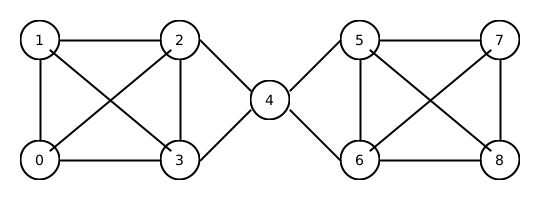
\includegraphics[width=0.5\linewidth]{z51.png}  
\end{figure}
$\kappa(G) = 1,\hspace{1cm} \lambda(G) =2,\hspace{1cm} \delta(G) = 3$\\\\
\noindent \textbf{DEF:} \\
$\lambda(G)$ - Spójność krawędziowa grafu spójnego $G=(V,E)$, \\ 
\indent $\lambda(G) = min \{|Y|: (Y \subseteq E) \land (G\textbackslash Y$ nie jest spójny$)\}$\\\\
$\delta(G)$ - Minimalny rząd wierzchołka grafu:\\
\indent $\delta(G) = min\{deg(x) : x \in V(G)\}$\\\\
$\kappa(G)$ - Spójność wierzchołkowa grafu spójnego:\\
\indent $\kappa(G)$ = 
$\begin{cases}
n - 1  & \text{: G \textasciitilde $K_{n}$}\\
min\{|X| : X \subseteq V \land G \textbackslash X$ nie jest spójny$   & \text{: nie jest pełny} 
\end{cases}$
,gdzie $K_{n}$ - graf pełny\\\\
\section{\centering Zadanie 52}
Załóżmy że $\lambda(G) = k > 0$ Pokaż, że jest rozbicie $\{U,V\}$ zbioru wierzchołków grafu takie, że jest dokładnie k krawędzi z jednym końcem w zbiorze $U$ i drugim w zbiorze $V$\\\\
ODP: \\
Usuwam k krawędzi i mam podział na 2 grafy\\\\\
\noindent \textbf{DEF:} \\
rozbicie - podzielenie wierzchołków z $G$ na dwa zbiory $\{U,V\}$ i ``usunięcie'' krawędzi między nimi, \\
$\lambda(G)$ - Spójność krawędziowa grafu spójnego $G=(V,E)$, \\ 
\indent $\lambda(G) = min \{|Y|: (Y \subseteq E) \land (G\textbackslash Y$ nie jest spójny$)\}$\\\\
\section{\centering Zadanie 55}
Niech $G$ będzie spójnym grafem w którym wszystkie wierzchołki mają rząd parzysty. Pokaż że $\lambda(G) \geq 2$ (czyli że usunięcie jednej dowolnej krawędzi nie rozspójnia grafu)\\\\
ODP:\\
Z tw Eulera, gdyby $\lambda(G) = 1$ to suma wszystkich stopni wierzchołków w każdym z utworzonych podgrafów byłaby nieparzysta, co jest nieprawdą\\\\
\noindent \textbf{DEF:} \\
\textbf{TW Eulera} - suma stopni wierzchołków jest parzysta w dowolnym grafie.\\
$\lambda(G)$ - Spójność krawędziowa grafu spójnego $G=(V,E)$, \\ 
\indent $\lambda(G) = min \{|Y|: (Y \subseteq E) \land (G\textbackslash Y$ nie jest spójny$)\}$\\\\
\section{\centering Zadanie 57 }
Podzielmy w dowolny sposób talię 52 kart na 13 grup po 4 karty. Pokaż, że z każdej z tych grup można wybrać po jednej karcie w taki sposób aby otrzymać zestaw 2, 3, 4, 5, 6, 7,8, 9, 10, W, K, D, A (nie ważne jakiego koloru).\\\\
ODP:\\
Tworzymy graf dwudzielny:
\begin{figure}[H]
	\centering
	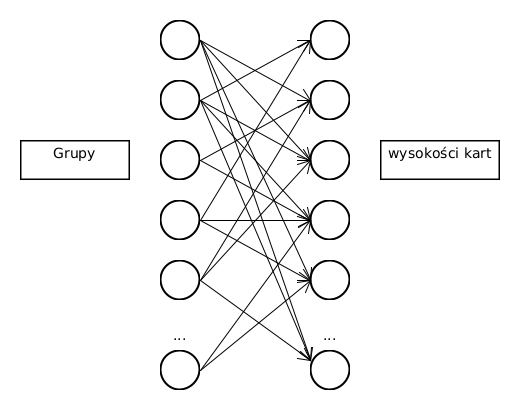
\includegraphics[width=0.5\linewidth]{z57.png}  
\end{figure}
\noindent graf ten ma maksymalnie 4 połączenia z podzbioru Grup do podzbioru wysokości kart\\
Z tw. Hall'a - każdy z podzbiorów grup ma co najmniej 1 połączenie z wysokościami\\\\
\noindent \textbf{DEF:} \\
\textbf{TW Hall'a} - Niech $G=G(A,B)$ będzie grafem dwudzielnym. Następujące warunki są równoważne:
\begin{enumerate}
	\item istnieje pełne skojarzenie w grafie $G$ z $A$ do $B$
	\item $(\forall X \subseteq A)(|X| \leq |\mathcal{N}(X)|)$
\end{enumerate}
\textbf{$\mathcal{N}$ określamy} - dla $G = G(D,C)$ i $X \subseteq D$ mamy $\mathcal{N}(X) = \{y \in C : (\exists x \in X)(\{x,y\} \in E(G))\}$\\
\textbf{Skojarzenie pełne} - Pełnym skojarzeniem (z $C$ do $D$) w grafie dwudzielnym $G=G(C,D)$ nazywamy dowolną różnowartościową funkcję $f:D\rightarrow C$ taką, że $(\forall x \in D)(\{x,f(x)\} \in E(G))$
\section{\centering Zadanie 61 // do uzupełnienia}
Niech $S = (S_{1}, S_{2},..., S_{m})$ będzie ciągiem zbiorów.\\ \textbf{Transwersala} tego ciągu zbiorów nazywamy ciąg $(s_{1},s_{2},...,s_{m})$ parami różnych elementów taki, że $s_{i} \in S_{i}$ dla każdego $i=1,...,m$.\\ Pokaż że rodzina S ma transwersalę wtedy i tylko wtedy, gdy:\\\\
$(\forall T \subseteq \{1,...,m\})(|\bigcup_{t\in T}S_{t}| \geq |T|)$\\\\
ODP:\\
\begin{figure}[H]
	\centering
	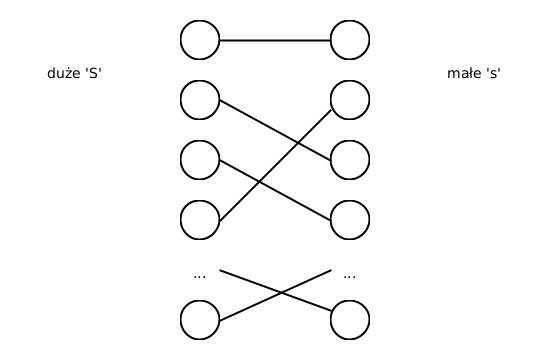
\includegraphics[width=0.5\linewidth]{z61.png}  
\end{figure}
\noindent Rodzina S będzie mieć transwersalę gdy znajdę pełne skojarzenie, czyli z \textbf{tw Hall'a}\\
$T = X$ z Hall'a \\ 
$\mathcal{N}(X) = \bigcup_{t\in T}S_{t}$ \\
$(\forall T \subseteq \{1,...,m\})(|\bigcup_{t\in T}S_{t}| \geq |T|)$\\\\
\noindent \textbf{DEF:} \\
\textbf{TW HALL'A}: \\
\begin{enumerate}
	\item istnieje pełne skojarzenie w grafie $G$ ($G=G(A,B)$) z $A$ do $B$
	\item $(\forall X \subseteq A)(|X| \leq |\mathcal{N}(X)|)$ \\\\
\end{enumerate}
\textbf{$\mathcal{N}$ określamy} - dla $G = G(D,C)$ i $X \subseteq D$ mamy $\mathcal{N}(X) = \{y \in C : (\exists x \in X)(\{x,y\} \in E(G))\}$\\
\textbf{d-d:}\\
Weźmy graf dwudzielny $G = G(A, B)$\\
Zdefiniujmy bijekcje $a: S \rightarrow A$ i $b: \bigcup_{S_i \in S} S_i \rightarrow B$\\
$(\forall x \in A \forall y \in B)((x,y) \in E(G) \Leftrightarrow b^{-1}(y) \in a^{-1}(x))$\\
Wtedy każdy element transwersali $s_i = b^{-1}(f(a(S_i)))$, gdzie $f: A \rightarrow B$ jest pełnym skojarzeniem\\
Dlatego transwersala istnieje wtedy i tylko wtedy, kiedy istnieje pełne skojarzenie f\\
Z twierdzenia Hall'a wiemy że pełne skojarzenie f istnieje wtedy i tylko wtedy, kiedy $(\forall X \subseteq A)(|X| \leq |\mathcal{N}(X)|) \equiv (\forall T \subseteq {1, ..., m})(|T| \leq |\bigcup_{t \in T} S_t|)$\\
\section{\centering Zadanie 62}
Pokaż, że każdy dwudzielny i regularny graf ma doskonałe skojarzenie.\\
\textbf{d-d:}\\
Weźmy $r$-regularny graf dwudzielny $G = G(A,B)$\\
$\sum_{a \in A} deg(a) = \sum_{b \in B} deg(b)$ bo dwudzielny\\
$(\forall v \in A \cup B)(deg(v) = r)$ bo $r$-regularny\\
więc $|A| * r = |B| * r$, czyli $|A| = |B|$\\
wtedy dowolne pełne skojarzenie musi być doskonałe\\
pełne skojarzenie $f: A \rightarrow B$ istnieje wtedy i tylko wtedy, kiedy $(\forall X \subseteq A)(|X| \leq |\mathcal{N}(X)|)$ (tw. Hall'a)\\
$(\forall X \subseteq A)(\sum_{x \in X} deg(x) \leq \sum_{y \in \mathcal{N}(X)} deg(y))$ co daje $(\forall X \subseteq A)(\sum_{x \in X} r \leq \sum_{y \in \mathcal{N}(X)} r)$\\
więc $(\forall X \subseteq A)(|X| \leq |\mathcal{N}(X)|)$\\
\section{\centering Zadanie 63 // do uzupełnienia}
Grupa złożona ze 100 studentów (s) ma uczestniczyć w egzaminach ustnych. Zespół egzaminacyjny składa się z 25 osób. Każdy student ma być przepytany przez jedną osobę z zespołu egzaminacyjnego. Wiadomo, że każdy ma co najmniej 10 ulubionych osób. Pokaż,że można ustawić sesję egzaminacyjną tak, aby (1) każdy student przepytany był przez ulubioną przez niego osobę (2) każdy egzaminator przepyta co najwyżej 10 studentów.\\\\
ODP:\\
\begin{figure}[H]
	\centering
	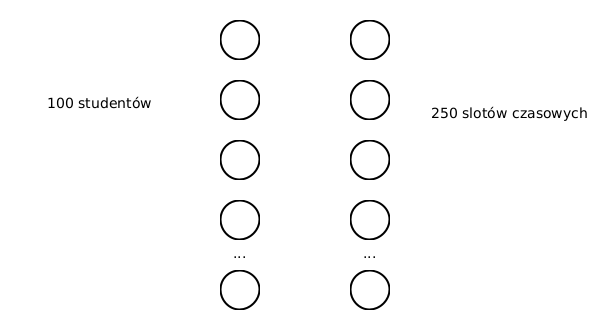
\includegraphics[width=0.5\linewidth]{z63.png}  
\end{figure}
Tworzymy graf dwudzielny jak powyżej. Wtedy $|\mathcal{N}(X)|$ to liczba przydzielonych prowadzących do grupy studentów.
\section{\centering Zadanie 74}
Niech $G = (\{0, ..., 19\},E)$, gdzie $E = \{(k,(k^{2}+1)$ mod $20) : k = 0, ..., 19\}$. Wyznacz silne komponenty spójne grafu oraz zredukowany graf acykliczny grafu $G$. \\\\
ODP: \\
Silnie spójny komponent : cykl $1 \rightarrow 2 \rightarrow 5 \rightarrow 6 \rightarrow 17 \rightarrow 10 \rightarrow 1$\\
\begin{figure}[H]
	\centering
	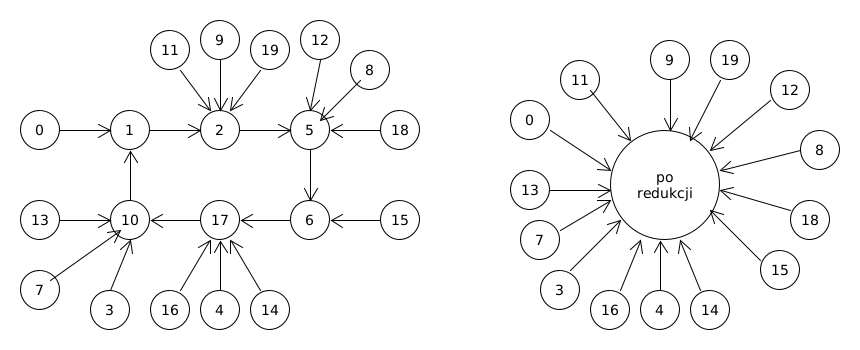
\includegraphics[width=1.0\linewidth]{z74.png}  
\end{figure}
\noindent \textbf{DEF}:\\
\textbf{Graf jest silnie spójny, jeśli} dla każdej pary wierzchołków x,y istnieje ścieżka od x do y.\\ 
\textbf{Podzbiór $\subseteq$ E jest silnie spójny jeśli} obcięcie grafu G do X jest grafem silnie spójnym. \\ \textbf{Silnie spójną składową nazywamy} maksymalny w sensie inkluzji silnie spójny podzbiór zbioru wierzchołków. \\\\
\textbf{Kondensacja grafu G} jest skierowanym grafem acyklicznym (dag).\\
\textbf{Kondensacja grafu skierowanego krok po kroku} - ustalamy digraf $G = (V,E,\phi)$:
\begin{enumerate}
	\item definiujemy $x>>y$ $\equiv$ istnieje ścieżka z x do y
	\item definiujemy $()x \equiv y) \leftrightarrow ((x >> y) \land (y >> x))$
	\item pokazujemy że $\equiv$ jest relacją równoważności na V
	\item na $V/\equiv$ definiujemy $E' = \{(C_{1},C_{2}) : (\exists e \in E)(fst(e) \in C_{1} \land snd(e) \in C_{2})\}$\\
	$\bullet$ $fst(e),snd(e)$ - pierwszy i drugi element krawędzi (jeżeli $e = (x,y)$ to $fst(e)=x,snd(e) = x$)\\\\
	Graf $(V/\equiv,E')$ to kondensacja grafu G
\end{enumerate}
\section{\centering Zadanie 75}
Niech $G$ będzie zorientowanym grafem acyklicznym o $n$ wierzchołkach. Pokaż, że graf ten ma co najwyżej $\binom{n}{2}$ krawędzi. Podaj przykład takiego grafu o dokładnie $\binom{n}{2}$ krawędziach.\\\\
ODP: \\
Graf skierowany acykliczny, o największej ilości krawędzi i $n$ wierzchołków:
\begin{enumerate}
	\item Z grafu o $|V| = n$ wierzchołkach weźmy $v_{0}$, ilość krawędzi które można z niego poprowadzić to $n-1$
	\item Weźmy teraz kolejny $V_{1}$, można poprowadzić co najwyżej $n-2$ krawędzi (nie można do samego siebie ani do $v_{0}$ bo powstanie cykl), i dalej analogicznie
	\item Suma wszystkich krawędzi to $\sum_{i=1}^{n-1}i=\frac{(n-1) \cdot n}{2}$
\end{enumerate}
$\binom{n}{2}$ po przekształceniu:\\
$\binom{n}{2} = \frac{n!}{(n-2) \cdot 2!} = \frac{n \cdot (n-1)}{2}$
\section{\centering Zadanie 78}
Niech $G$ będzie grafem skierowanym o $n$ wierzchołkach i $m$ krawędziach.
\begin{enumerate}
	\item Pokaż, że jeśli $G$ jest spójny to $n-1\leq m \leq n(n-1)$
	\item Pokaż, że jeśli $G$ jest silnie spójny to $n\leq m \leq n(n-1)$\\\\
\end{enumerate}
ODP: \\
Z poprzedniego zadania: \\
Maksymalna liczba krawędzi w grafie prostym to $\binom{n}{2}$\\
(1) Minimalna liczba krawędzi w grafie spójnym to $n-1$ (graf liniowy)\\
(2) Minimalna liczba krawędzi w grafie spójnym to $n$ (graf cykliczny)\\\\

\noindent \textbf{DEF:}\\
\textbf{Graf prosty} nie ma pętli i krawędzi wielokrotnych.\\
\textbf{Graf spójny}, to graf w którym dla każdej pary wierzchołków istnieje ścieżka, która je łączy.\\
\textbf{Graf jest silnie spójny}, jeżeli każde dwa wierzchołki są osiągalne jeden z drugiego.

\end{document}
